\chapter{Introduction}
\label{ch:Introduction}

	In the financial markets around the world, derivative instruments can be derived from Sixth Century B.C. Renowned philosopher of Greece; Thalus is thought to be the first person that had formulated a deal, which is alike to that of option derivative of today, for making profit.
A derivative is a security with a price that is dependent upon or derived from one or more underlying assets.
The derivative itself is a contract between two or more parties based upon the asset or assets.
 Value of a derivative changes with price change of its underlying asset (share, commodity, currency and many more). With the passage of time, the need of these instruments increased among various sections of the society for hedging purposes. Later, the speculative motive of the investors also surfaced and led to its popularity.\\[0.5cm]
Considering the given situation, pricing options is very important for the financial markets. In order to solve that issue, the use of mathematical techniques is a force of thing for formulating of the pricing of the option contracts. Mathematical models have been used in economics for a long time. By now, operations research, econometrics and time series analysis constitute major parts of curricula of business schools and economics departments.
Therefore, we will go into the complexity of the financial market to see how it needs some our  mathematical techniques .

\section{The structure of the financial market }
\fontsize{11pt}{20pt}\selectfont In the financial markets of economic system, we have found out two different sectors. They are household who saves money and business who needs money for the purpose of prodution or sale of goods and services. Financial market acts as an intermediary between the savers and investors of money where traders buy and sell stocks, bonds, derivatives, foreign exchange and commodies.\\[0.5cm]
There are three conditions to classifying market. Firstly, based on working capital, we have primary market where the new security issues sold to initial buyers. Typically involves an investment bank who underwrites the offering and second market where Securities previously issued are bought and sold. Involves both brokers and dealers. Secondly, based on operating approach, markets be assigned by exchange market that Stock trades conducted via centralized place. Buy/sell is conducted through the exchange; no direct contract between seller and buyer and OTC market (Over-The-Counter) where no centralized place. Trading is done directly between two parties, without the supervision of an exchange. Lastly, based on goods, there are stock market, bond market and derivative instrument. Let's look at stock market, a financial market that enables investors to buy and sell shares of publicly traded companies. There are common stock and preferred stock. Then bond market, a financial market where participants can issue new debt  or buy and sell debt securities. The form may be bonds, notes, bills, and so on. For derivative instrument, a financial market that trades securities that derive its value from its underlying asset including stock right, warrant, option. In this research, options will be analized for deriving the formula.  
\section{Options}
Options are a type of derivative security. They are a derivative because the price of an option is intrinsically linked to the price of something else. Specifically, options are contracts that grant the right, but not the obligation to buy or sell an underlying asset at a set price on or before a expiration date. The right to buy is called a call option and the right to sell is a put option. A call option, might be thought of as a deposit for a future purpose, is bought if the trader expects the price of the underlying to rise within a certain time frame. For example, let's say you purchase a call option on shares of Intel (INTC) with a strike price which is a fixed at which an asset may be bought or sold of $\$40$ and an expiration date of May 16th. This option would give you the right to purchase 100 shares of Intel at a price of $\$40$ on May 16th (the right to do this, of course, will only be valuable if Intel is trading above $\$40$ per share at that point in time) and you will pay option premium for the writer. Conversely, a put option is bought if the trader expects the price of the underlying to fall within a certain time frame.  \\[0.5cm]
At a premium, since the writer of an option is exposed to potential liabilities in the future, he must be compensated with an up-front premium paid by the holder who has bought this option when they together enter into the option contract.  When you buy an option, the purchase price is called the premium. If you sell, the premium is the amount you receive. The premium isn't fixed and changes constantly. The premium is likely to be higher or lower today than yesterday or tomorrow. Changing prices reflect the give and take between what buyers are willing to pay and what sellers are willing to accept for the option. The point of agreement becomes the price for that transaction. \\ [0.5cm]
In addition, options can be categorized based on the method in which they are traded, their expiration cycle, and the underlying security they relate to. It is listed of some different common types of option: Barrier,
American, European, Asian, Lookback... This research will be focus into the combination of European and Barrier option that is more attractive and cheaper than the respective standard European options. 
	\subsection{European option}
	European options are contracts that give the holder the right but not the obligation, to buy or sell the underlying security at a specific price (the strike price) only on the option's expiration date. As the exercise date is limited in the European option, it removes the uncertainty about possible early execution. The lack of this uncertainty is expected to encourage more investors to trade stock options. Theoretically, a European option has lower value than an otherwise, it is because a European option does not enjoy the convenience that arises from flexibility in timing of exercise, which is a premium option. The holder must pay a premium at the initial time. This option is the path independent option. \\ [0.5cm]
	The path independent option whose payoff depends solely on the events specified to take place upon expiration, rather than the path taken by the underlying variable (price, rate, index, etc). An example for European option, if an investor buys a call option with a strike price of $\$20$, he would benefit if the underlying rises above $\$20$ upon expiration. If not, he would not exercise and the premium paid to buy the option is lost. We consider the payoffs for a European option that is value at the expiration time, as a function of the underlying stock price	
	\begin{center}
Call option = $\max(S-K,0)$\\
Put option = $\max(K-S,0)$\\
	\end{center}
Where\\
$S$: the current price\\
$K$: the strike price   \\[0.5cm]
Let's look at the following diagram which discribes profit of call option. Suppose that we have one call option with exercise price $\$50$ which costs $\$5$, the stock price moves from $\$0$ to $\$100$.  
\begin{figure}[htp]
	\begin{center}
		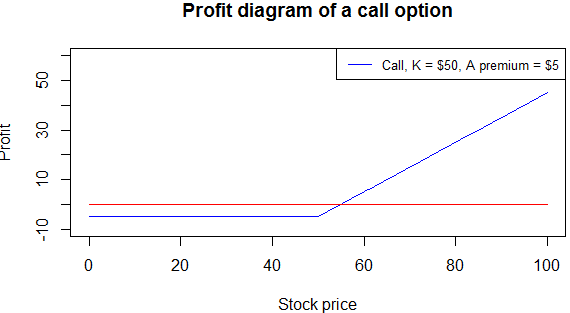
\includegraphics[scale=0.8]{Rplot02}
	\end{center}
	\label{refRplot02}
	\caption{Profit of a call option}
\end{figure}

The above diagram implies that if the stock price belows the strike price, the holder would not exercise the option and had to pay a premium of $\$5$. Conversely, if the stock price is higher than the strike price and differences between two of them is greater than zero, he would practice the option and receive profit which is equal to the stock price minus the strike price and a premium. 
	
	\subsection{Barrier option}
	The barrier option is the simpiest popular path dependent option. It is a type of option and its distinctive feature is that the payoff depends not
	only on the final price of the underlying asset, but also on whether the asset price has
	breached some barrier level during the life of the option. So, a barrier option’s payoff depends on two price levels:
	the strike price and the so-called barrier price. One of the important things is that the holder of the option may be compensated
	by a rebate payment for the cancellation of the option, that helps to keep losing all premium he paid before. Let's consider two most common types of barrier options are knock-out and knock-in barrier options. 	
	\begin{itemize}
		\item Knock-out barrier options is a type of barrier option becomes worthless if the underlying asset price touches the barrier. Moreover, it is also devided into two parts, down and out barrier option which implies if the underlying asset's price falls below the barrier at any point in the option's life, the option will be worthless and up and out barrier option which implies if the underlying asset’s price increases above the barrier at any point in the option’s life, the option will be worthless.
			
	\item Knock-in option has no value until the underlying asset price crosses the in-barrier. This option is classified as down and in barrier option which means if the underlying asset price moves below a barrier at any point in the option’s life, the option comes into existence and up and in barrier option which indicates if the price of the underlying asset rises above the barrier at any point in the option’s life, the option comes into existence.	
	\end{itemize}
Barrier options carry a higher risk to the holder than the more standard types of contracts. With a knock out contract,  the holder carries the risk of their investment basically ceasing to exist if the underlying security moves significantly and reaches the knock out price. With a knock in contract, if the underlying security only moves a little in price there may be no profits to be taken. There is, however, one significant advantage that barrier options offer traders, barrier options are generally cheaper than contracts that do not include a barrier price  because of the increased risk that the holder has to take.  The barrier options are popular and attractive thanks to benefits that they give investors more flexibility to express their view on the asset price movement in the option contract. The buyer can achieve {\itshape option premium reduction} through the barrier provision by not paying a premium to cover scenarios he or she views as unlikely. The option writer can limit liabilities when the asset price rises acutely. 
	\subsection{European barrier call option}
	It is a type of option including characters of both European option and barrier option which means the option will be exercised at expiration date unless the underlying asset price reached or exceeded a lower barrier during the option's life. Especially, the option cannot be activated again if the underlying asset price go up after down to a lower barrier. The distinctive features of call options and put options are just conversely like one is the right to buy the asset and hence benefit would be gained as the price of the underlying goes up and one is the right to sell the asset and hence benefit would be gained as the price of the underlying goes down. Therefore, we will focus on only one side and the call option will be analyzed.\\
		\begin{figure}[htp]
		\begin{center}
			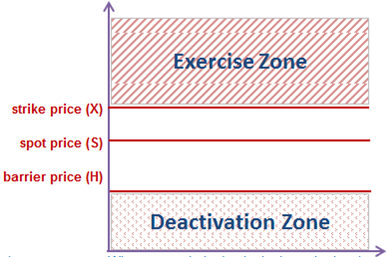
\includegraphics[scale=0.9]{figure1}
		\caption{Down and Out Call option $X > H$}
		\label{reffig1} 
	    \end{center}
     	\end{figure} \\
    Let's look at Figure ~\ref{reffig1}  which decribes Down and Out Call option when the strike price $(X)$ is greater than the barrier $(H)$. Expectation of the price will go up over the strike price to exercise option and make payoff is equal difference between the stock price at expiration date and the strike price. If the price goes down, the option will be deactivated.   
	\subsection{European barrier call option with rebates}
	This is a specified of European barrier call option which a knock-out occurs, the holder of the option will receive a partial rebate on the premium paid to the option writer. European barrier call option with rebates are cheaper than the respective standard European options because a zero payoff maybe occur before expiry time T. Lower premiums are usually offered for more exotic barrier option, which make them particularly attractive to hedgers in the financial market.\\[0.5cm]
	Let's illustrate this type of option by an example. We consider the European down-and-out call option under the underlying asset of XYZ stock, the current price is approximately, $\$39$ and rebate is $\$5$. If the XYZ price falls to $\$28$ which is a barrier level within the next six months. the writer will have to  pay $\$5$ dollars for the holder if XYZ stock is less than or equal to $\$28$ at any point in the next six months.